\documentclass[11pt,a4paper]{article}

\usepackage[utf8]{inputenc}
\usepackage[T1]{fontenc}
\IfFileExists{lmodern.sty}{\usepackage{lmodern}}{}
\IfFileExists{french.ldf}{\usepackage[french]{babel}}{}
\usepackage[margin=2.6cm]{geometry}
\usepackage{xcolor}
\usepackage[most]{tcolorbox}
\usepackage{booktabs,tabularx,array}
\usepackage{enumitem}
\usepackage{tikz}
\usetikzlibrary{arrows.meta,positioning}
\usepackage[hidelinks]{hyperref}
\setlength{\parskip}{0.5em}
\setlength{\parindent}{0pt}
\setlength{\emergencystretch}{3em}

\definecolor{bleu}{RGB}{40,90,160}
\definecolor{bleuclair}{RGB}{232,240,250}
\definecolor{gris}{RGB}{110,115,125}

% Encadré « En résumé »
\newtcolorbox{resume}{breakable, enhanced, colback=bleuclair, colframe=bleu,
  boxrule=0.5pt, arc=2pt, left=8pt, right=8pt, top=6pt, bottom=6pt,
  title={\small\bfseries En résumé}, coltitle=white, colbacktitle=bleu}

% Encadré « Exemple »
\newtcolorbox{exemple}{breakable, enhanced, colback=white, colframe=gris!60,
  boxrule=0.4pt, arc=2pt, left=8pt, right=8pt, top=4pt, bottom=4pt,
  title={\small\bfseries Exemple}, coltitle=black, colbacktitle=gris!15}

\title{\textbf{Le modèle V-LSTM expliqué simplement}\\[4pt]
\large Une probabilité de hausse pour décider quand acheter et quand vendre}
\author{Alexandre Berlia}
\date{Octobre 2026}

\begin{document}
\maketitle

\noindent\textit{Ce document s'adresse à un lecteur qui connaît les marchés mais pas
l'apprentissage automatique. Il ne contient ni formule ni code. La version technique, avec
les équations et la correspondance avec les programmes, est un document séparé.}

\setcounter{tocdepth}{1}
\tableofcontents
\newpage

% ===========================================================================
\section{En bref}
% ===========================================================================
Chaque jour, le modèle donne pour chaque titre suivi \textbf{une probabilité de hausse}
sur les semaines suivantes, par exemple : « 62\,\% de chances que XLK soit plus haut dans
22 séances qu'aujourd'hui ». Des règles simples transforment ensuite ce chiffre en
décision : acheter, garder ou vendre.

Pour produire ce chiffre, le modèle fait ce que ferait un analyste technique discipliné :
\begin{enumerate}[nosep]
  \item il regarde quels signaux techniques se sont déclenchés récemment (un RSI qui
  remonte, un cours qui sort des bandes de Bollinger\dots) ;
  \item il tient compte du \textbf{climat économique}, mesuré par un score macroéconomique ;
  \item il compare la situation du jour à des milliers de situations passées, et regarde
  ce qui s'est produit ensuite.
\end{enumerate}

La différence avec un analyste humain : le modèle a « vu » près de vingt ans d'historique,
il applique toujours la même méthode, et il apprend lui-même quels signaux comptent et
dans quel contexte.

\begin{resume}
\begin{itemize}[nosep]
  \item \textbf{Ce qu'il produit} : une probabilité de hausse par titre et par jour.
  \item \textbf{Ce qu'il ne produit pas} : un objectif de cours, ni l'ampleur de la hausse.
  Le modèle dit si le titre sera plus haut, pas de combien.
  \item \textbf{Ce qu'on en fait} : on achète quand la probabilité est nettement élevée,
  on vend quand elle retombe.
\end{itemize}
\end{resume}

\begin{figure}[h]
\centering
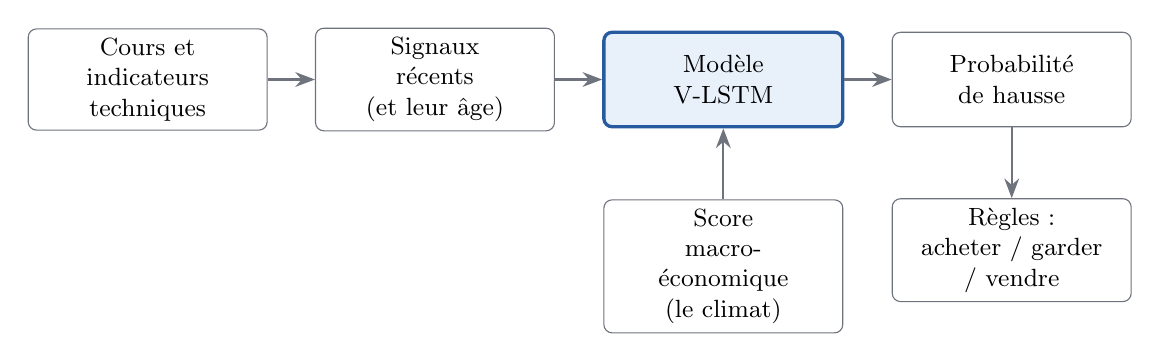
\begin{tikzpicture}[
  node distance=6mm and 6mm,
  boite/.style={draw=gris, rounded corners=3pt, align=center, font=\small,
                minimum height=12mm, text width=28mm, fill=white},
  cle/.style={boite, draw=bleu, very thick, fill=bleuclair},
  fl/.style={-{Stealth[length=2.5mm]}, gris, thick}]
  \node[boite] (donnees) {Cours et\\indicateurs\\techniques};
  \node[boite, right=of donnees] (signaux) {Signaux\\récents\\(et leur âge)};
  \node[cle, right=of signaux] (modele) {Modèle\\V-LSTM};
  \node[boite, right=of modele] (proba) {Probabilité\\de hausse};
  \node[boite, below=9mm of modele] (score) {Score\\macro-\\économique\\(le climat)};
  \node[boite, below=9mm of proba] (regles) {Règles :\\acheter / garder\\/ vendre};
  \draw[fl] (donnees) -- (signaux);
  \draw[fl] (signaux) -- (modele);
  \draw[fl] (modele) -- (proba);
  \draw[fl] (score) -- (modele);
  \draw[fl] (proba) -- (regles);
\end{tikzpicture}
\caption{La chaîne complète, des cours à la décision.}
\end{figure}

% ===========================================================================
\section{Ce que le modèle regarde}
% ===========================================================================
\subsection{Des signaux techniques plutôt que des niveaux}
Le modèle ne regarde pas « le RSI vaut 52 ». Il regarde \textbf{des événements} : « le RSI
vient de repasser au-dessus de 45 ». C'est la façon dont un praticien lit ses
indicateurs : ce qui compte est le franchissement d'un seuil, pas le niveau exact.

Six indicateurs sont suivis, chacun avec une règle d'achat et une règle de vente, soit
douze signaux au total :

\begin{center}
\small
\begin{tabularx}{\linewidth}{@{}l >{\raggedright\arraybackslash}X >{\raggedright\arraybackslash}X@{}}
\toprule
\textbf{Indicateur} & \textbf{Signal plutôt favorable} & \textbf{Signal plutôt défavorable} \\
\midrule
RSI                     & repasse au-dessus de 45 & repasse sous 65 \\
Bandes de Bollinger (\%B) & remonte au-dessus de 0 (retour dans les bandes par le bas) & redescend sous 0,95 \\
Rendement sur 5 jours   & dépasse +3\,\% & passe sous $-2{,}5$\,\% \\
Stochastique            & remonte au-dessus de 15 & redescend sous 75 \\
MACD (histogramme)      & remonte au-dessus de $-2{,}5$ & redescend sous 2,5 \\
Efficacité de tendance (ER) & dépasse 0,35, cours au-dessus de celui d'il y a 10 jours & repasse sous 0,35, cours en dessous de celui d'il y a 10 jours \\
\bottomrule
\end{tabularx}
\end{center}

Ces seuils sont fixés à la main, à partir de l'expérience. Le modèle ne les modifie pas :
il apprend seulement \textbf{quel poids accorder à chacun}.

\subsection{L'âge du signal compte}
Un signal d'il y a deux jours n'a pas la même valeur qu'un signal d'il y a deux semaines.
Chaque signal est donc noté selon sa \textbf{fraîcheur} : 1 le jour où il se déclenche, puis
une valeur qui diminue de moitié tous les deux jours, et 0 au bout de dix séances.

\begin{center}
\small
\begin{tabular}{lccccccc}
\toprule
Séances depuis le signal & 0 & 1 & 2 & 3 & 4 & 5 & plus de 10 \\
\midrule
Fraîcheur & 1 & 0,71 & 0,50 & 0,35 & 0,25 & 0,18 & 0 \\
\bottomrule
\end{tabular}
\end{center}

\begin{exemple}
Lundi, le RSI de XLK repasse au-dessus de 45 : ce signal vaut 1. Mercredi, il vaut 0,5.
La semaine suivante, il ne vaut presque plus rien. Si un second signal favorable apparaît
mercredi (le stochastique remonte au-dessus de 15), le modèle voit deux signaux récents en
même temps, ce qui pèse plus qu'un signal isolé.
\end{exemple}

\subsection{Quelques repères sur les prix}
En plus des signaux, le modèle voit quelques mesures simples : la performance du titre
sur 1, 5 et 20 jours, sa volatilité récente et le volume du jour comparé à sa moyenne.

\subsection{Le climat économique}
Le dernier ingrédient est un \textbf{score macroéconomique mensuel}, construit à partir
d'indicateurs avancés de l'économie américaine : enquêtes de la Fed de Philadelphie,
indice d'activité de la Fed de Chicago, ISM manufacturier, PMI de Chicago, permis de
construire, créations d'emplois, inflation PCE, chômage et production industrielle. Un
score bas (sous 25) signale un climat dégradé, un score élevé (au-dessus de 75) un climat
porteur.

Le score n'est utilisé qu'une fois réellement publié : celui d'un mois donné n'entre dans
le modèle qu'un mois après la fin de ce mois. On évite ainsi d'utiliser une information
qu'on n'aurait pas eue à l'époque.

% ===========================================================================
\section{Comment il raisonne}
% ===========================================================================
Le nom « V-LSTM » désigne deux briques. On peut les comprendre comme deux réflexes d'un
analyste expérimenté.

\subsection{Premier réflexe : trier les signaux (la partie « V »)}
Face à douze signaux, un bon analyste ne les traite pas tous de la même façon. Certains
jours, le retour dans les bandes de Bollinger est le signal le plus parlant ; d'autres
jours, c'est la tendance de fond. La première brique du modèle fait ce tri : chaque jour,
elle \textbf{répartit 100\,\% d'attention} entre les signaux, par exemple 30\,\% sur le RSI,
25\,\% sur Bollinger, 5\,\% sur le MACD, et ainsi de suite.

Cette répartition change d'un jour à l'autre et peut être consultée après coup. C'est
l'un des intérêts du modèle : on peut voir \textbf{sur quoi il s'est appuyé}, ce qui n'est
pas le cas de la plupart des réseaux de neurones.

\subsection{Deuxième réflexe : se souvenir de l'enchaînement (la partie « LSTM »)}
Un analyste ne regarde pas seulement la séance du jour. Il regarde comment la situation a
évolué : « le RSI est remonté il y a trois jours, puis le stochastique a suivi hier ». La
seconde brique lit les \textbf{20 dernières séances dans l'ordre}, comme on lit un graphique de
gauche à droite, et retient ce qui est utile. Elle a une mémoire qui sait conserver une
information importante et oublier ce qui est devenu obsolète.

\subsection{Le climat change la lecture}
Le score macroéconomique ne s'ajoute pas comme un treizième signal. Il agit comme une
\textbf{toile de fond} qui change la façon de lire les signaux. Un RSI qui remonte dans une
économie en expansion n'a pas la même portée que le même RSI en pleine récession. Le
modèle peut donc apprendre qu'un signal compte beaucoup dans un climat porteur et peu dans
un climat dégradé.

\subsection{Un modèle commun à tous les titres}
Le même modèle sert pour tous les titres suivis. Cela lui donne beaucoup plus d'exemples
de chaque signal : un retour dans les bandes de Bollinger sur trente titres pendant douze
ans représente des milliers de cas. En contrepartie, il lit un signal de la même façon sur
un titre technologique et sur un titre cyclique.

\begin{resume}
Le modèle trie les signaux du jour, lit leur enchaînement sur les 20 dernières séances,
tient compte du climat économique, et en tire une probabilité de hausse.
\end{resume}

% ===========================================================================
\section{Comment il apprend}
% ===========================================================================
\subsection{Par l'exemple}
On ne donne au modèle aucune règle du type « si le RSI remonte, achète ». On lui montre
des milliers de situations passées, chacune avec sa réponse : « 22 séances plus tard, le
titre était-il plus haut ? ». Au début, ses probabilités sont quelconques. À chaque
erreur, il ajuste légèrement ses réglages internes pour se tromper un peu moins. Après des
milliers d'ajustements, il a appris quelles combinaisons de signaux étaient, dans le passé,
suivies d'une hausse.

\subsection{Trois périodes séparées, dans l'ordre du temps}
L'historique est découpé en trois périodes qui ne se chevauchent pas :

\begin{center}
\small
\begin{tabularx}{\linewidth}{@{}l l >{\raggedright\arraybackslash}X@{}}
\toprule
\textbf{Période} & \textbf{Dates} & \textbf{Rôle} \\
\midrule
Apprentissage & 2005 -- 2016 & le modèle apprend sur ces exemples \\
Validation    & 2017 -- 2019 & on règle la stratégie (les seuils d'achat et de vente) \\
Test          & 2020 -- aujourd'hui & on mesure le résultat final, une seule fois \\
\bottomrule
\end{tabularx}
\end{center}

C'est l'équivalent d'un examen : on n'évalue pas un élève sur les exercices qu'il a déjà
corrigés. La période de test n'est jamais utilisée pour régler quoi que ce soit ; c'est
la seule qui donne une idée honnête de ce que le modèle aurait fait « en vrai ».

\subsection{Ne jamais regarder le futur}
Le piège principal en finance est d'utiliser, sans s'en rendre compte, une information
qu'on n'avait pas à la date de la décision. Plusieurs précautions l'évitent : le score
macro n'est utilisé qu'après sa publication ; les dernières séances de chaque période sont
écartées, pour qu'aucun exemple d'apprentissage ne « déborde » sur la période suivante ; les
mises à l'échelle des données sont calculées sur la période d'apprentissage seulement.

\subsection{S'arrêter au bon moment}
Un modèle qui s'entraîne trop longtemps finit par apprendre par cœur les particularités
de son historique au lieu des régularités utiles. C'est le \textbf{surapprentissage}, comme
un étudiant qui mémorise les annales sans comprendre le cours. Pour l'éviter, on vérifie
après chaque passage sur les données si le modèle s'améliore aussi sur la période de
validation, qu'il n'a pas apprise. Dès qu'il cesse de progresser pendant huit passages, on
s'arrête et on garde la meilleure version.

% ===========================================================================
\section{De la probabilité à la décision}
% ===========================================================================
\subsection{Deux seuils}
La probabilité seule ne dit pas quoi faire. Deux seuils la transforment en ordres :
\begin{itemize}[nosep]
  \item \textbf{seuil d'achat} : on achète quand la probabilité le dépasse, par exemple 62\,\% ;
  \item \textbf{seuil de sortie} : on vend quand elle retombe en dessous, par exemple 50\,\%.
\end{itemize}
Ces seuils ne sont pas choisis au hasard : on teste plusieurs combinaisons sur la période
de validation et on retient celle qui donne le meilleur rapport entre rendement et risque,
après frais. On vérifie aussi que des seuils voisins donnent des résultats proches : un
réglage qui ne fonctionne que pour une valeur précise est probablement un coup de chance.

\subsection{Un stop de protection (optionnel)}
On peut ajouter un stop : la ligne est vendue si le cours baisse de plus de deux fois
l'ATR (la variation quotidienne moyenne du titre) sous le prix d'achat. Le stop s'adapte
donc à la volatilité de chaque titre. Il est activable ou non selon le besoin.

\subsection{Les règles du portefeuille}
\begin{itemize}[nosep]
  \item Le capital est découpé en \textbf{parts égales} (10 au plus). Chaque achat investit
  une part ; les parts non utilisées restent en liquidités.
  \item Au plus \textbf{deux achats par jour}, en commençant par les probabilités les plus élevées.
  \item Au plus \textbf{deux lignes par titre} : si un nouveau signal d'achat apparaît au
  moins trois séances après le premier achat, sans signal de vente entre-temps, on peut
  renforcer la position.
  \item On sort quand la probabilité passe sous le seuil de sortie (toutes les lignes du
  titre), ou sur le stop. Il n'y a pas de durée de détention fixe.
\end{itemize}

\begin{exemple}
Lundi, la probabilité de Schneider passe à 64\,\%, au-dessus du seuil d'achat de 62\,\% : on
achète une part. Vendredi, quatre séances plus tard, un nouveau signal porte la probabilité
à 66\,\% : on achète une deuxième part. Trois semaines après, la probabilité retombe à
48\,\%, sous le seuil de sortie de 50\,\% : on vend les deux lignes.
\end{exemple}

\subsection{Acheter au cours qui a servi à décider}
Le modèle est lancé en séance, par exemple à 17\,h. Le cours de 17\,h sert à la fois à
calculer la probabilité et à acheter. On évite ainsi d'acheter le lendemain à
l'ouverture, à un prix qui peut être très différent (le « gap »).

% ===========================================================================
\section{Comment juger les résultats}
% ===========================================================================
\subsection{La qualité des probabilités}
Le premier indicateur est l'\textbf{AUC}. Il répond à la question : « si je prends au hasard
un jour de hausse et un jour de baisse, le modèle donne-t-il une probabilité plus forte au
jour de hausse ? ». Une AUC de 0,50 correspond au hasard (pile ou face), 1,00 à un modèle
parfait.

\textbf{Sur les marchés, une AUC de 0,52 à 0,55 est déjà un bon résultat.} Les prix sont
très difficiles à prévoir, et un léger avantage répété sur des centaines de décisions peut
suffire. Une AUC annoncée de 0,70 sur des actions doit au contraire faire soupçonner une
erreur, en général l'utilisation involontaire d'une information future.

\subsection{La comparaison avec la référence}
La stratégie est comparée à une référence simple : \textbf{acheter les mêmes titres et les
garder}, frais compris. Attention à comparer ce qui est comparable :

\begin{exemple}
Sur 2020 -- 2026, XLK acheté et conservé rapporte environ 19\,\% par an. La stratégie
rapporte 5\,\% par an, mais elle n'est investie que 30\,\% du temps. Investie 30\,\% du temps
\emph{au hasard}, elle aurait rapporté environ $0{,}30 \times 19 \approx 5{,}7$\,\%. Le
rendement brut ne dit donc pas grand-chose : il faut regarder le rendement obtenu pendant
qu'on est investi et le risque pris.
\end{exemple}

\subsection{Les indicateurs à regarder}
\begin{center}
\small
\begin{tabularx}{\linewidth}{@{}l >{\raggedright\arraybackslash}X@{}}
\toprule
\textbf{Indicateur} & \textbf{Question à laquelle il répond} \\
\midrule
Ratio de Sharpe & combien de rendement par unité de risque ? C'est le critère principal. \\
Perte maximale & quelle a été la pire baisse depuis un plus haut ? \\
Exposition moyenne & quelle part du temps le capital est-il investi ? \\
Rendement rapporté à l'exposition & les jours choisis sont-ils meilleurs que la moyenne ? \\
Nombre de trades & y a-t-il assez de décisions pour que le résultat soit significatif ? \\
Taux de trades gagnants & quelle part des opérations finit en gain ? \\
\bottomrule
\end{tabularx}
\end{center}

Sur un seul titre en forte hausse, comme un ETF technologique, une stratégie qui sort
souvent du marché bat rarement « acheter et conserver » en rendement. Son intérêt, s'il
existe, se voit dans un meilleur rapport rendement/risque et une perte maximale plus
faible. Le gain le plus probable vient d'un univers de plusieurs titres, où le modèle peut
choisir \emph{lesquels} acheter, et pas seulement \emph{quand}.

% ===========================================================================
\section{Limites et risques}
% ===========================================================================
\begin{itemize}
  \item \textbf{Le passé ne garantit pas l'avenir.} Le modèle a appris sur 2005 -- 2016. Si
  le marché change durablement de comportement, ses probabilités peuvent se dégrader.
  \item \textbf{Le risque de chance déguisée.} Tester trente réglages et garder le meilleur
  produit presque toujours un beau résultat, même sans aucun vrai pouvoir prédictif. C'est
  pourquoi les réglages sont choisis sur la validation et le test n'est regardé qu'une fois.
  \item \textbf{Peu de décisions.} Sur un seul titre, la stratégie ne fait que quelques trades
  par an. Sur trois ans, l'incertitude sur le ratio de Sharpe est d'environ $\pm 0{,}6$ : un
  résultat peut paraître bon ou mauvais par simple hasard.
  \item \textbf{La direction, pas l'ampleur.} Le modèle prévoit si le titre montera, pas de
  combien. Il peut avoir souvent raison et manquer les quelques mois qui font l'essentiel
  de la performance, par exemple un rebond violent après une chute, quand les signaux sont
  encore mauvais.
  \item \textbf{Les frais.} Chaque aller-retour coûte. Un avantage faible peut disparaître
  si la stratégie trade trop souvent.
  \item \textbf{Une lecture identique pour tous les titres.} Le modèle commun lit un signal
  de la même façon sur un titre cyclique et sur un titre technologique.
\end{itemize}

% ===========================================================================
\section{Une journée type}
% ===========================================================================
\begin{enumerate}
  \item \textbf{Vers 17\,h}, on relève le dernier cours de chaque titre.
  \item On lance le programme. Il ajoute la séance du jour à l'historique, recalcule les
  indicateurs et les signaux, puis calcule la probabilité de hausse de chaque titre.
  \item Il compare ces probabilités aux seuils et aux lignes déjà détenues, et affiche trois
  listes : \textbf{à vendre} (avec le motif : signal ou stop), \textbf{à garder} et
  \textbf{à acheter} (nouvelle ligne ou renforcement).
  \item On passe les ordres au cours du moment.
  \item On met à jour la liste des lignes détenues (titre, date et prix d'achat) pour le
  lendemain.
\end{enumerate}
Le modèle lui-même n'est pas réentraîné chaque jour. Il est entraîné une fois, puis
réutilisé tel quel ; on ne le réentraîne que si l'on change les signaux, les dates ou les
règles.

% ===========================================================================
\section*{Petit glossaire}
\addcontentsline{toc}{section}{Petit glossaire}
% ===========================================================================
\begin{description}[style=nextline, leftmargin=1.5em, itemsep=2pt]
  \item[Apprentissage automatique] Méthode où un programme apprend des règles à partir
  d'exemples, au lieu qu'on les lui écrive.
  \item[ATR] Variation quotidienne moyenne d'un titre ; sert à placer un stop adapté à sa
  volatilité.
  \item[AUC] Note de 0,5 (hasard) à 1 (parfait) mesurant si le modèle classe bien les jours
  de hausse avant les jours de baisse.
  \item[Fraîcheur] Note de 0 à 1 indiquant depuis combien de temps un signal s'est déclenché.
  \item[Horizon] Durée sur laquelle porte la prévision ; ici 22 séances, environ un mois.
  \item[LSTM] Brique du modèle qui lit les dernières séances dans l'ordre et en garde la mémoire utile.
  \item[Probabilité de hausse] Chance estimée que le titre soit plus haut à l'horizon qu'aujourd'hui.
  \item[Ratio de Sharpe] Rendement obtenu par unité de risque (volatilité).
  \item[Score macroéconomique] Note mensuelle du climat économique, de 0 à 100 environ.
  \item[Seuil d'achat / de sortie] Niveaux de probabilité au-dessus desquels on achète et
  en dessous desquels on vend.
  \item[Surapprentissage] Défaut d'un modèle qui a appris par cœur son historique au lieu de
  règles générales ; il brille sur le passé et déçoit ensuite.
  \item[Validation / test] Périodes mises de côté : la première pour régler la stratégie,
  la seconde pour la juger une seule fois.
  \item[VSN] Brique du modèle qui répartit chaque jour l'attention entre les signaux.
\end{description}

\end{document}
